\chapter{Class 2 - Monday, January 23\ts{rd}, 2017}
\section{\S 3 Ordinary Differential Equations}
\begin{imp:defn}{Ordinary Differential Equation}{} Let $f(x)$ be a function of $x$ on interval $I$ then ODE involves $x,f(x)$ \& 1 or more derivatives of $f$. Order of an ODE is highest derivative of $f$.\\
Recall: $y=f(x)$ is solution of an ODE if when you plug in $y, y', y''...$ as necessary, equation holds.
\end{imp:defn}
\begin{imp:defn}{Explicit Definition of Solution}{} Let $y=f(x)$, define $y$ as a function of $x$ on $I$. $f(x)$ is an explicit solution (or simply a solution) if for all $x\in I$, $F(x, f(x), f'(x),...f^{(n)})=0$
\end{imp:defn}
\begin{ex}
\begin{align*}
    e^{x-y}+(e^{y-x})\dfrac{dy}{dx} & =0\\
    e^{2y}+e^{2x} & =1\\
    F(x, f(x), f'(x)=0 \rightarrow [(e^{x-f(x)})+(e^{f(x)-x})(f'(x)) & = 0]
\end{align*}
\begin{align*}
    \text{Look at: }e^{2y}+e^{2x} & = 1\\
    2\,\dfrac{dy}{dx}\, e^{2y}+2e^{2x} & = 0\\
    \dfrac{dy}{dx} & = \frac{-e^{2x}}{e^{2y}} = -e^{2x-2y}
\end{align*}
Now plug it into the ODE $$e^{x-y}+(e^{y-x})(-e^{2x-2y})=e^{x-y}-e^{x-y}=0$$
\end{ex}
\section{\S 4 General Solution of ODEs}
\begin{imp:defn}{Parameter}{} Let $y=f(\textcolor{red}{x}; \textcolor{blue}{c_1}, \textcolor{blue}{c_2}) = 2x+3+ c_1e^x+c_2e^{2x}$\\
   $ \textcolor{red}{x} \& \leftarrow \text{variable}$\\
    $\textcolor{blue}{c} \& \leftarrow \text{Parameters - Constants that vary with initial conditions}$
\end{imp:defn}
\begin{ex} Given an equation with parameters, how do you show it is or isn't a solution for an ODE? \textcolor{red}{Plug in, check if equals zero.}
\end{ex}
\begin{ex}
Given a solution, how do you determine an ODE for which the Solution satisfies?\\
\begin{align*}
    x^2-cy+c^2 &=0 \leftarrow c=\text{constant}\\
    2x-cy' &=0\\
    y' &= \frac{1}{c}*2x \leftarrow \text{if} c\neq 0\\
    \textcolor{red}{\text{Let's Square }} y'&=\frac{1}{c}*2x\\
    (y')^2&=\frac{4}{c^2}x^2\\
    \textcolor{red}{\text{Multiply Both Sides by }(y')^2 \rightarrow} (x^2-cy+c^2)(y')^2&=0\textcolor{red}{(y')^2}=0\\
    x^2(y')^2-cy(\frac{4}{c^2}x^2)+4x^2&=0\\
    \textcolor{red}{\text{Note: }\frac{4}{c}yx^2=2xy(\frac{2}{c}x)}&=\textcolor{red}{2xy(y')}\\
    \rightarrow x^2(y')^2-2xy*y'+4x^2&=0 \leftarrow \text{ is the ODE!}
\end{align*}
\end{ex}
\section{\S 4C Initial Conditions}
\begin{imp:defn}{Particular Solution}{} A particular solution of a differential equation satisfies the differential equation but also has no arbitrary constants.
\end{imp:defn}
\begin{note}
If we have $n$ parameters in a solution, we need $n$ initial conditions
\end{note}
\begin{ex}
Initial Condition $\rightarrow$ $y \left( 3 \right) =1$\\
\begin{align*}
    \dfrac{dy}{dx} & = y \\
    \text{ODE} \rightarrow y'-y & = 0\\
    \dfrac{dy}{dx} & =y\\
    1dy&= ydx\\
    \int \frac{1}{y}dy &=\int dx \text{ if } y\neq 0\\
    \ln \left| y \right| +c &=x+c\\
    \ln \left| y \right| &=x+c_1\\
    y &=e^{x+c_1}\\
    y &=e^{c_1}e^x=Ae^x\\
    \text{Use Initial Condition} \rightarrow 1&=Ac^3\\
    A &=e^{-3}\\
    y &= e^{x-3}
\end{align*}
\end{ex}
\section{\S Direction Fields}
\begin{note}
There should be a graph here.
\end{note}
Given $y=f(x)$ or $f(x,y)=0$ on $I$ and $y'$ is defined as $\dfrac{dy}{dx}=f'(x)$. Then $y'$ gives the slope of the graph of $f(x)$ at each point $x \in I$.
\begin{imp:defn}{Integral Curve}{} If $y=f(x)$ satisfies $y'=F(x,y)$ then graph of $f(x)$ called the integral curve.
\end{imp:defn}
\begin{ex}
How to draw direction field:
\begin{center}
 \begin{tabular}{|c||c|c|c|c|} 
 \hline
 \multicolumn{5}{|c|}{$y'=2x+y$} \\
 \hline
 x\backslash y & -1 & 0 & 1 & 2\\
 \hline\hline
 -1 & \textcolor{red}{-3} &  &  &  \\ 
 \hline
 0 &  &  &  &  \\
 \hline
 1 &  &  &  &  \\
 \hline
 2 &  &  &  &  \\
 \hline
\end{tabular}
\end{center}
Entries are $y'$ evaluated at $(x,y)$ point. \textcolor{red}{$y'(-1,-1)=2(-1)+(-1)=-3$}


 \begin{figure}[h!]

    \begin{subfigure}{\textwidth}
    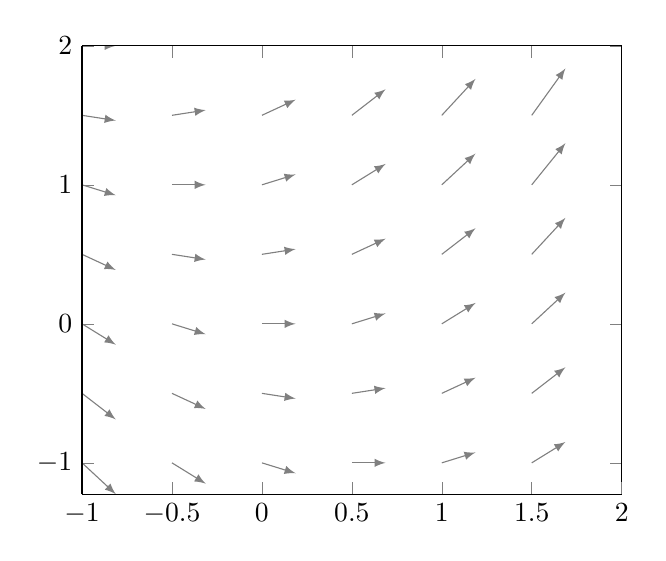
\begin{tikzpicture}

    \begin{axis}[
        view={0}{90},
        domain=-1:2,
        y domain=-1:2,
        xmax=2, ymax=2,
        samples=7
    ]
    \addplot3 [gray, quiver={u={2.5}, v={2*x+y}, scale arrows=0.075,
every arrow/.append style={-latex}}] (x,y,0);
    %\addplot [thick, red] table [x=x, y=y] {\loadedtable};
    \end{axis}
    \end{tikzpicture}
    
    \end{subfigure}

\end{figure}
\end{ex}